
% header %{{{1

\documentclass[tikz, border=1mm]{standalone}

\usepackage{amsmath}
\usepackage{tikz}

\usetikzlibrary{calc,angles,quotes}

% document %{{{1

% opening %{{{2

\begin{document}
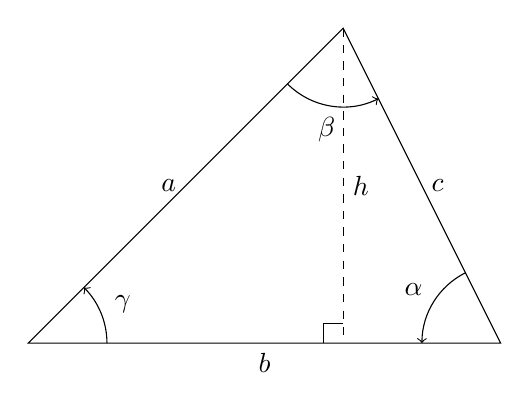
\begin{tikzpicture}[scale=1.0]

% coordinates %{{{2

	\coordinate (A) at (0,0);
	\coordinate (C) at (6,0);
	\coordinate (B) at (4,4);

	% feet of altitude from B to AC
	\coordinate (D) at (4,0);

% triangle %{{{2

	\draw (A) -- (B) -- (C) -- cycle;

	% altitude

	\draw[dashed] (B) -- (D);

% side labels %{{{2

	\node[left]  at ($(A)!0.5!(B)$) {$a$};
	\node[below] at ($(A)!0.5!(C)$) {$b$};
	\node[right] at ($(B)!0.5!(C)$) {$c$};

	% height label
	\node[right] at ($(B)!0.5!(D)$) {$h$};

% angles labels %{{{2

	\pic[draw, ->, "$\alpha$", angle eccentricity=1.3, angle radius=1cm]
	{angle = B--C--A};

	\pic[draw, ->, "$\beta$", angle eccentricity=1.3, angle radius=1cm]
	{angle = A--B--C};

	\pic[draw, ->, "$\gamma$", angle eccentricity=1.3, angle radius=1cm]
	{angle = C--A--B};

% right angle markers %{{{3

	\pic [draw, angle radius=7pt, angle eccentricity=1]
	{right angle = B--D--A};

% closing %{{{2

\end{tikzpicture}
\end{document}
